\documentclass[a4paper,12pt,twocolumn,landscape]{article}

\usepackage{superpack2015}
\usepackage{tkz-fct}
\usepackage{lscape}

\usepackage[heightrounded]{geometry}	% heightrounded permet d'afficher les footers correctement
\geometry{hmargin=0.5cm,vmargin=1.5cm}

\setlength{\columnseprule}{0.5pt}		% Ligne séparatrice milieu document
\setlength{\columnsep}{50pt}			% Espace de chaque côté de la ligne
\setlength{\headsep}{15pt}
\addtolength{\textheight}{20pt}
%\setlength{\textwidth}{770pt}
%\setlength{\hoffset}{20pt}

\classichf
	% Nom du style
	{activites}
	% Hauteur sous header
	% 14.5pt si une ligne (1 \baselineskip)
	% 29.0pt si deux lignes (2 \baselineskip)
	{14.5pt}
	% Head
	{}
	{\textbf{Activités}}
	{}
	% Foot
	{}
	{}
	{}

%\usepackage{showframe}
%\usepackage{layout}

\begin{document}
\pagestyle{activites}	%\thispagestyle{premierepage} pour isoler des styles de pages

\activite Le quadrilatère tournant

$ABCD$ représente une feuille au format~$A4$ c'est-à-dire un rectangle de côtés $AB = 29,7cm$ et $BC = 21cm$.\\
On place $M$ sur $[AB]$.\\
On place ensuite $N$ sur $[BC]$, $P$ sur $[CD]$ et $Q$ sur $[DA]$ tels que~:\\ $AM = BN = CP = DQ$

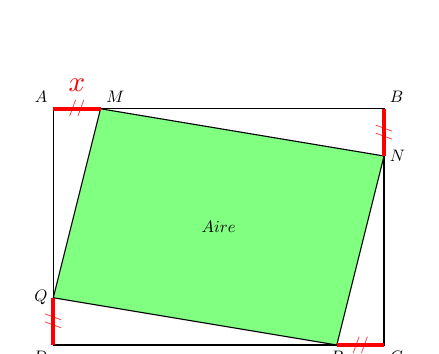
\begin{tikzpicture}[scale=0.6,every node/.style={scale=0.6}]
	\coordinate (A) at (0,0);
	\coordinate (B) at (7,0);
	\coordinate (C) at (7,-5);
	\coordinate (D) at (0,-5);
	\coordinate (M) at (1,0);
	\coordinate (N) at (7,-1);
	\coordinate (P) at (6,-5);
	\coordinate (Q) at (0,-4);
	\coordinate (S) at (7/2,-5/2);
	\draw (A) rectangle ++(7,-5);
	\draw (A)--(B)--(C)--(D)--cycle;
%	\draw [very thick,red] (A)--(M) node [midway,above] {$x$};
	\draw [black,fill=green!50] (M)--(N)--(P)--(Q)--cycle;
	\draw (A) node[above left] {$A$};
	\draw (B) node[above right] {$B$};
	\draw (C) node[below right] {$C$};
	\draw (D) node[below left] {$D$};
	\draw (M) node[above right] {$M$};
	\draw (N) node[right] {$N$};
	\draw (P) node[below] {$P$};
	\draw (Q) node[left] {$Q$};
	\draw (S) node {$Aire$};
%	\foreach \point in {A, B, C, D}
%		\draw (\point) node[above left] {$\point$};
	\draw [red,ultra thick] (A)--(M)node[midway,sloped]{$//$};
	\draw [red,ultra thick] (B)--(N)node[midway,sloped]{$//$};
	\draw [red,ultra thick] (C)--(P)node[midway,sloped]{$//$};
	\draw [red,ultra thick] (D)--(Q)node[midway,sloped]{$//$};
	\draw (0.5,0.5) node [scale=1.75,red] {$x$};
\end{tikzpicture}


L'aire verte peut-elle être égale à $300~cm^2$~?
\activite On propose les programmes de calcul suivants~:\\

\begin{minipage}{0.25\textwidth}
\noindent Choisir un nombre,\\
lui ajouter 4,\\
multiplier le résultat par 5.\\[1em]
On trouve $35$.\\[1em]
Quel était le nombre de départ~?\\
\end{minipage}
\begin{minipage}{0.25\textwidth}
\noindent Choisir un nombre,\\
lui ajouter 4,\\
multiplier le résultat par 5,\\
ajouter le nombre de départ.\\[1em]
On trouve $62$.\\[1em]
Quel était le nombre de départ~?
\end{minipage}


\paragraph*{Activités 3 à 7}~\\

\noindent Le carré $ABCD$ a un côté de longueur 8 cm.\\
$M$ est un point du segment $[AB]$.\\
On dessine dans le carré $ABCD$ :
\begin{itemize}
	\item Un carré de côté $[AM]$
	\item Un triangle isocèle de base $[MB]$ et dont la hauteur a même mesure que le côté $[AM]$ du carré.
\end{itemize}
Trois dessins sont proposés pour trois positions différentes du point $M$.\\


\def\echelle{0.8}
\def\couleur{red!50}
\begin{tikzpicture}[scale=\echelle,every node/.style={scale=\echelle}]
	\coordinate (A) at (0,0);
	\coordinate (B) at (4,0);
	\coordinate (C) at (4,4);
	\coordinate (D) at (0,4);
	\coordinate (M) at (1,0);
	\draw (A)--(B)--(C)--(D)--cycle;
	\draw[fill=\couleur] (A) rectangle (1,1);
	\draw[fill=\couleur] (M) -- (2.5,1) -- (B) -- cycle;
	\draw[dashed] (1,1) -- (4,1);
	\draw (M) node[below] {$M$};
	\draw (A) node[below left] {$A$};
	\draw (B) node[below right] {$B$};
	\draw (C) node[above right] {$C$};
	\draw (D) node[above left] {$D$};
\end{tikzpicture}
\begin{tikzpicture}[scale=\echelle,every node/.style={scale=\echelle}]
	\coordinate (A) at (0,0);
	\coordinate (B) at (4,0);
	\coordinate (C) at (4,4);
	\coordinate (D) at (0,4);
	\coordinate (M) at (2,0);
	\draw (A)--(B)--(C)--(D)--cycle;
	\draw[fill=\couleur] (A) rectangle (2,2);
	\draw[fill=\couleur] (M) -- (3,2) -- (B) -- cycle;
	\draw[dashed] (2,2) -- (4,2);
	\draw (M) node[below] {$M$};
	\draw (A) node[below left] {$A$};
	\draw (B) node[below right] {$B$};
	\draw (C) node[above right] {$C$};
	\draw (D) node[above left] {$D$};
\end{tikzpicture}
\begin{tikzpicture}[scale=\echelle,every node/.style={scale=\echelle}]
	\coordinate (A) at (0,0);
	\coordinate (B) at (4,0);
	\coordinate (C) at (4,4);
	\coordinate (D) at (0,4);
	\coordinate (M) at (3,0);
	\draw (A)--(B)--(C)--(D)--cycle;
	\draw[fill=\couleur] (A) rectangle (3,3);
	\draw[fill=\couleur] (M) -- (3.5,3) -- (B) -- cycle;
	\draw[dashed] (3,3) -- (4,3);
	\draw (M) node[below] {$M$};
	\draw (A) node[below left] {$A$};
	\draw (B) node[below right] {$B$};
	\draw (C) node[above right] {$C$};
	\draw (D) node[above left] {$D$};
\end{tikzpicture}

\activite Dans quelle situation a-t-on l'aire du triangle la plus grande ?
\activite Dans quelle situation l'aire du carré est égale à celle du triangle ?
\activite Dans quelle situation l'aire du motif est elle égale à la moitié de celle de ABCD ?
\activite Dans quelle situation a-t-on l'aire du triangle supérieure à la moitié de celle du carré ?
\activite Comment évolue l'aire du motif en fonction de AM ? en fonction de MB ?


\end{document}


%
%%\exercicebareme{4}
%\exercicebareme{6}
%\exercicebareme{10}
%\exerciceunpoint
%\exercicebonus
%\FIN
%\BONNESVACANCES
%\BONCOURAGE
%\hrulefill